%\chapter{Desenvolvimento}
\label{desenvolvimento}
\section{Remoção na Arvore Sequencial}
    Iniciando o desenvolvimento da prática, as arvores foram criadas na IDE assim como os vetores de tamanhos diversos para armazenar os valores que serão inseridos na arvore. Porém, o Java não permite a criação de vetores em 10\textsuperscript{9} elementos, então todas as arvores criadas, foram geradas até 10\textsuperscript{7} elementos. A partir disso, foram utilizados métodos de inserção de dados da Pratica 3, desenvolvida anterior a esta, já que este trabalho trata-se de uma continuação direto com estudos sobre remoção.
    
    A os dados selecionados para a remoção foram gerados utilizando a biblioteca interna do Java "Random", que permitiu gerar valores aleatórios entre 0 e n (n = quantidade de elementos), aumentando a taxa de sucesso para gerar valores validos para a remoção.
    Os dados apresentados a seguir inicialmente trazem os resultados do tempo de execução da da remoção de 5\% de elementos aleatórios de arvores de diferentes tamanhos que receberam seus valores de forma ordenada:
    
    \begin{center}
        \begin{tabular}{| l | r |}
            \hline
            Quantidade de elementos & Tempo em Nanossegundos\\
            \hline
            10\textsuperscript{1} & 3700\\
            10\textsuperscript{3} & 820800\\
            10\textsuperscript{5} & 832481000\\
            10\textsuperscript{7} & 8880000000000\\
            \hline
        \end{tabular}
    \end{center}

        \begin{center}
            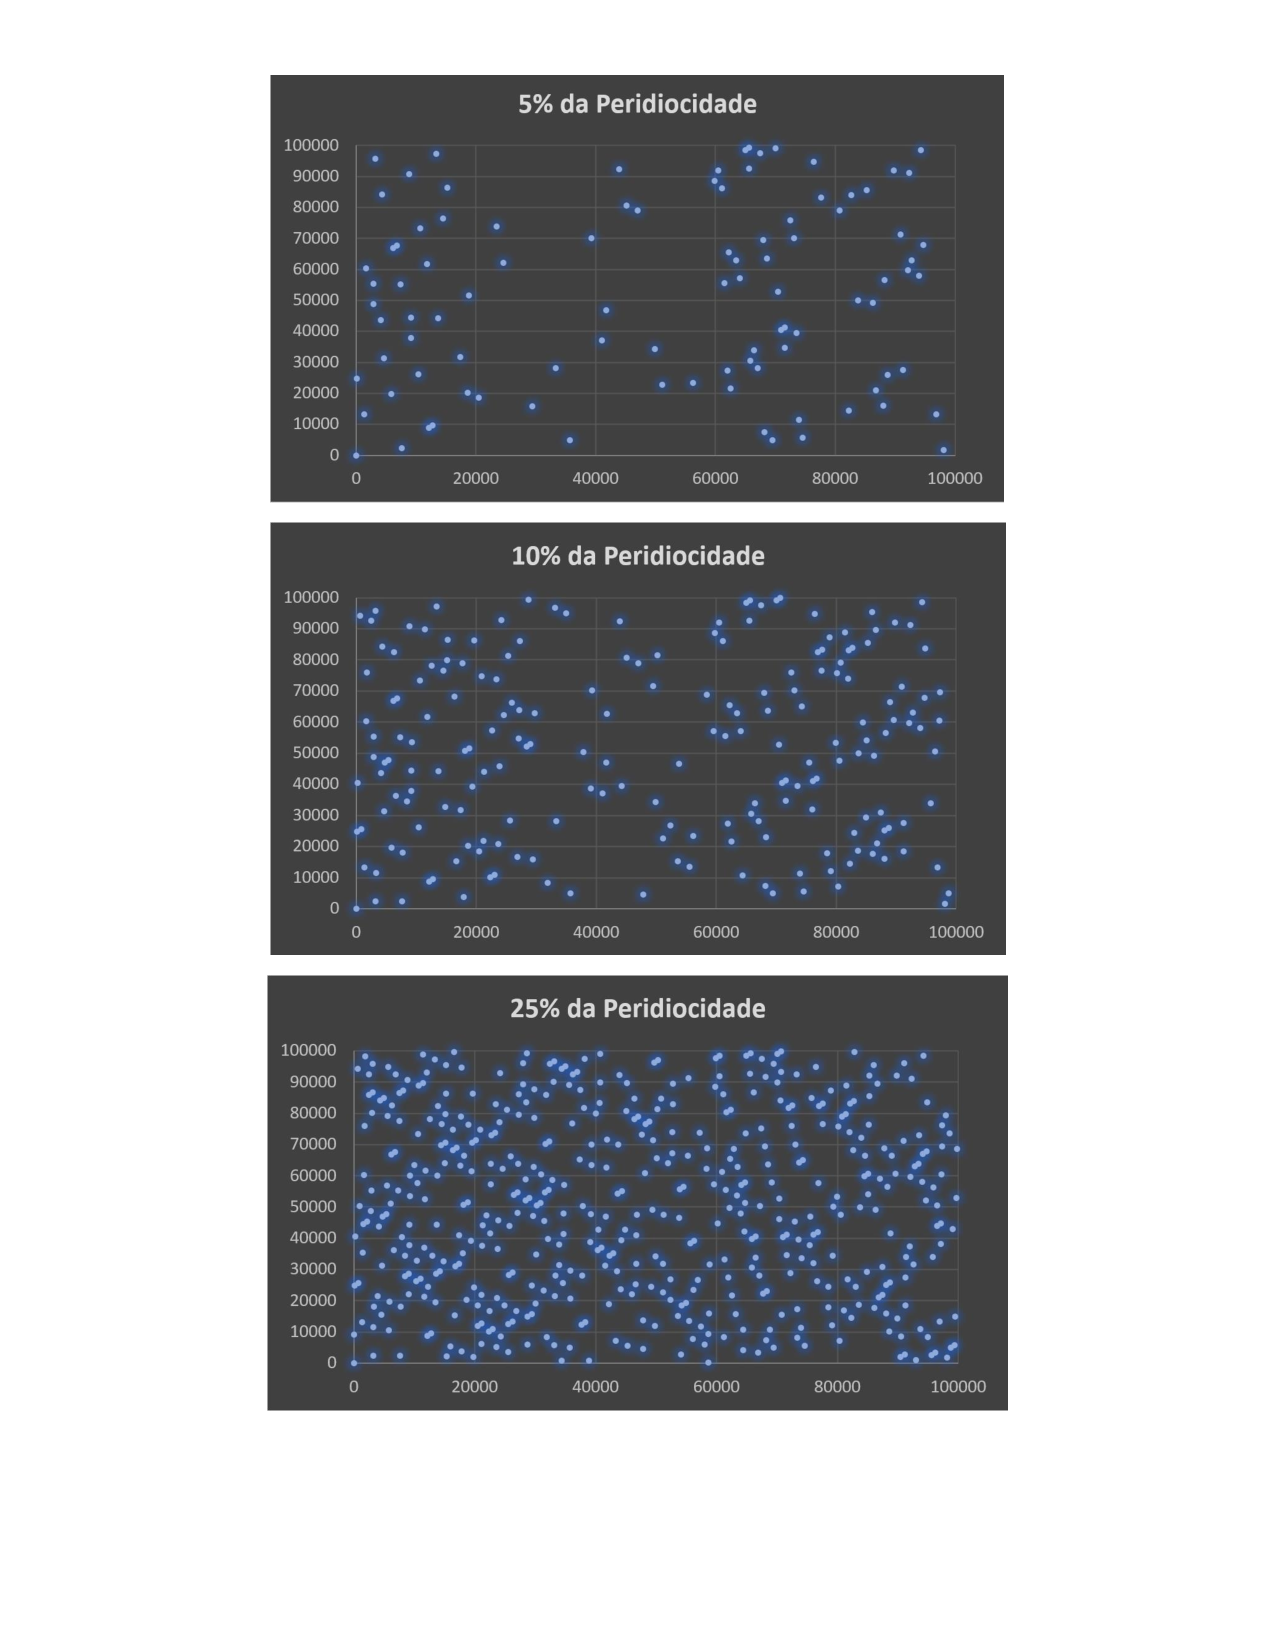
\includegraphics[scale=0.8]{Trabalho AED/fig/fig1.pdf}
            \label{fig:Grafico 1}
        \end{center}

\section{Remoção na Arvore Randômica}

Para a remoção de elementos aleatórios desta arvore foi gerado um vetor com valores aleatórios utilizando um gerador congruencial pseudo aleatório com os seguintes parâmetros:
        \begin{center}
        Semente = 0;
       
        Modulo = 1073741824;
       
        Multiplicador = 843314861;
       
        Incremento = 453816693;
        \end{center}

estes parâmetros também foram utilizados na inserção, então é certo que os mesmos estarão na arvore, mas não foram removidos na mesma ordem que foram inseridos, e sim de forma aleatória também.

Logo os dados apresentados a seguir trazem os resultados do tempo de execução da da remoção de 5\% de elementos aleatórios de arvores de diferentes tamanhos que receberam seus valores de forma aleatória:

\begin{center}
        \begin{tabular}{| l | r |}
            \hline
            Quantidade de elementos & Tempo em Nanossegundos\\
            \hline
            10\textsuperscript{1} & 68300\\
            10\textsuperscript{3} & 320100\\
            10\textsuperscript{5} & 2681900\\
            10\textsuperscript{7} & 160521900\\
            \hline
        \end{tabular}
    \end{center}
    
    \begin{center}
            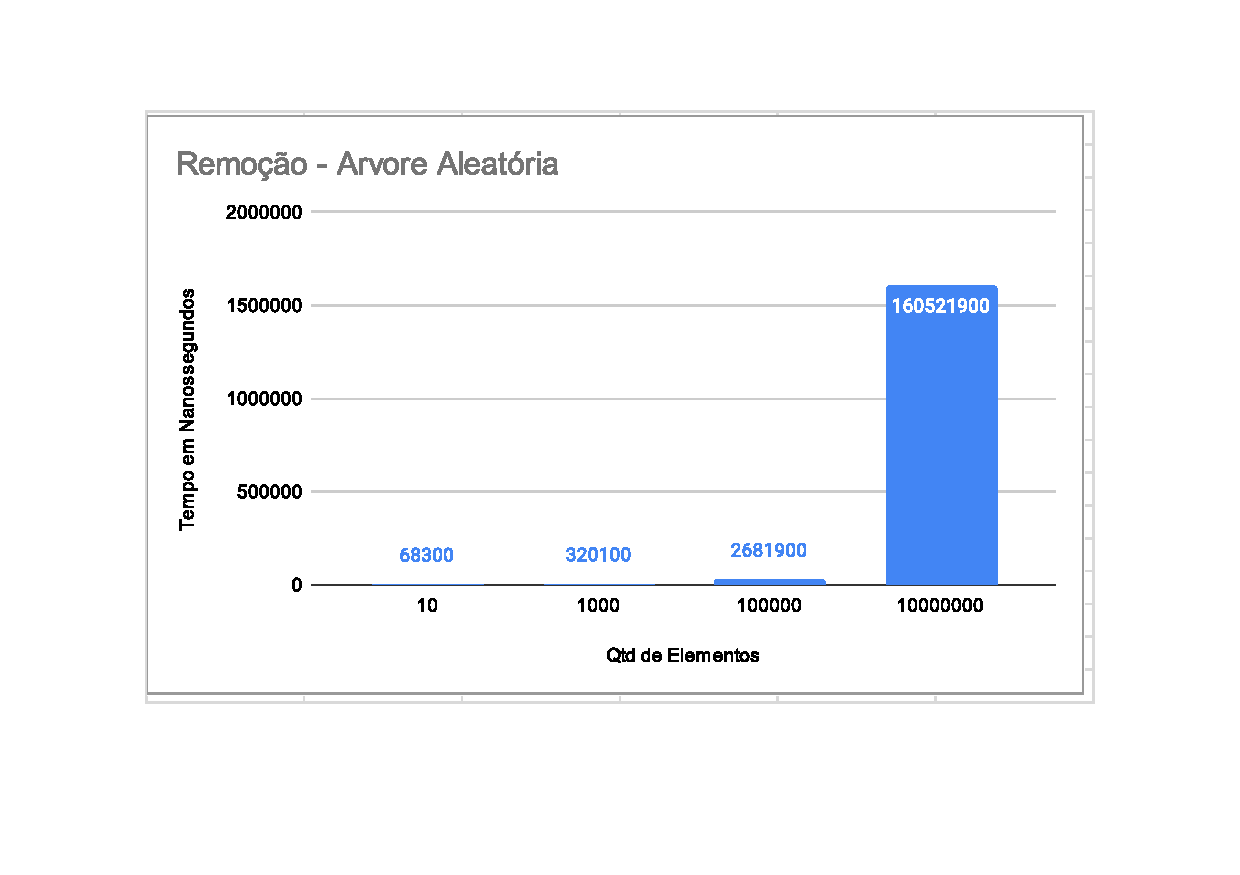
\includegraphics[scale=0.8]{Trabalho AED/fig/fig2.pdf}
            \label{fig:Grafico 2}
    \end{center}
    
\section{Remoção na Arvore Balanceada}
Para a remoção de elementos de dentro da arvore balanceada a logica utilizada segue a mesma da arvore sequencial, já que os valores inseridos na mesma estão entre 0 e n (n = quantidade de elementos), porem foram inseridos em uma condição especial que força a arvore a ser formada de já balanceada, como foi visto na atividade pratica 3.

Logo os dados apresentados a seguir trazem os resultados do tempo de execução da remoção de 5\% de elementos aleatórios de arvores balanceadas de diferentes tamanhos:

    \begin{center}
        \begin{tabular}{| l | r |}
            \hline
            Quantidade de elementos & Tempo em Nanossegundos\\
            \hline
            10\textsuperscript{1} & 4300\\
            10\textsuperscript{3} & 6900\\
            10\textsuperscript{5} & 989400\\
            10\textsuperscript{7} & 191030400\\
            \hline
        \end{tabular}
    \end{center}
    
    \begin{center}
            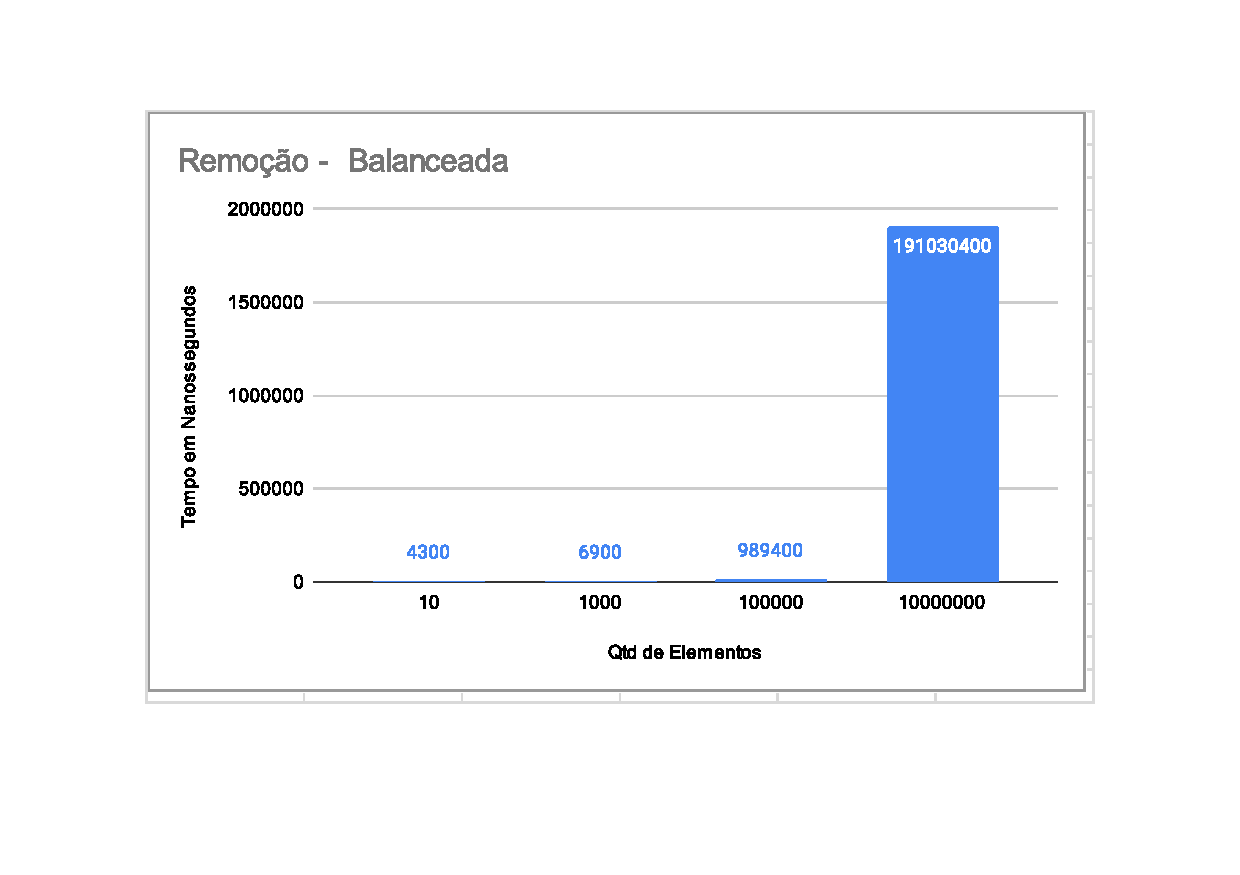
\includegraphics[scale=0.8]{Trabalho AED/fig/fig3.pdf}
            \label{fig:Grafico 3}
    \end{center}
\pagebreak
